\documentclass[11pt,conference]{IEEEtran}
\usepackage[utf8]{inputenc}
\usepackage[english]{babel}
\usepackage{graphicx}
\graphicspath{ {images/} }

\begin{document}

\section{Experiments}
To build a training set, the three of us each performed all seven gestures three times. In our testing set, we all performed each gesture only once. While we believed at the time that this would be sufficient, as we are all of very different builds, it actually proved to be insufficient, as we will explain later.

We performed these gestures while the data acquisition program was running, allowing us to construct primitive data files. We then fed these data files into the second program, the formatter, to produce a model that could be used with libSVM. In our final product, this provided an accuracy of about 80\%.

We did encounter some difficulty in acquiring this data. In some of our initial trials, while we were in proper range for the Kinect to read our skeletons in a neutral position, our hands and arms would be out of the frame when raised. Also, sometimes the Kinect would simply not detect our forms, and we would have to redo the experiment.

We produced three testing sets, each of us went through all of the gestures once to produce a testing set. These were the sets that were used to obtain the accuracy of our gesture detection. Our results found the accuracy to be 80.9524\%. The results show that the program struggled with telling the difference between gestures 2(right arm out) and 4(right arm up). This is most likely due to our relatively small training set.

\begin{figure}[h]
\caption{Confusion Matrix}
\centering
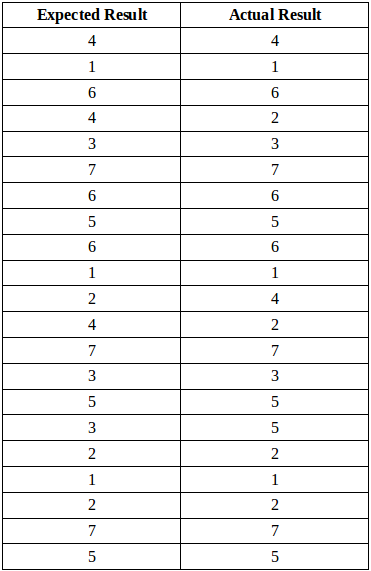
\includegraphics[width=\linewidth]{confusion_matrix}
\end{figure}

In order to get the accuracy of our gesture detection, we obtained our training and testing sets produced by the second program. We then used the easy.py program in libSVM to read these files and obtain the accuracy and the optimal C and gamma values. These values were found to be 8192.0 and 0.03125 respectively. To further increase our accuracy we experimented with different numbers of bins in the histograms from the second program. We found that 11 bins gave us optimal results.

\begin{figure}[h]
\caption{graph of the grid search}
\centering
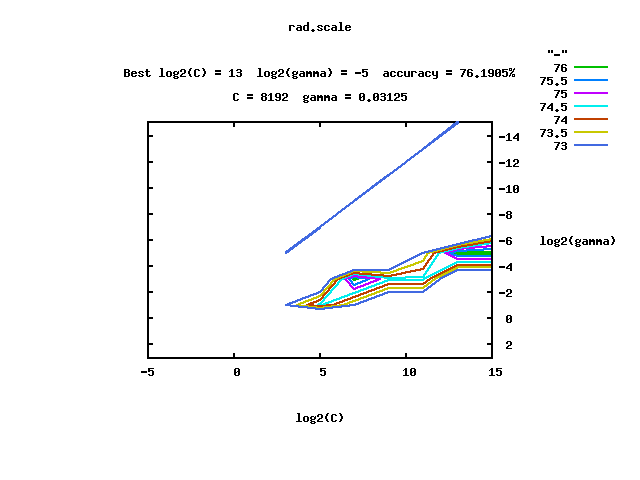
\includegraphics[width=\linewidth]{scale}
\end{figure}

Finally, we ran our program with the game space invaders. We found the gestures with the right hand seamed to work well, but there was difficulty with detecting gestures with the left hand. Again, this was most likely due to our small training set. Given a larger training set we are confident that our program would work much better.


\end{document}